\section{The Fabry-Perot Interferometer}
Optical resonators were utilized as helpful gadgets as early as 1899, when Fabry and Perot depicted the utilization of a parallel-plate resonator as a multipass interferometer. Part of the incident light on this Fabry– Perot resonator is transmitted and another part is reflected, with power divisions that rely upon numerous factors. A simple illustration of the basic Fabry-Perot is shown in Figure 2.1, here $r_{1} t_{1}$ are the reflectivity constant and transmitivity constant of the mirror 1 respectively and $r_{2} t_{2}$ are the reflectivity and transmitivity constants of the mirror two respectively. Also, $E_{i}$ is the incident Electromagnetic energy, $E_{t}$ is the transmitted energy and $E_{r}$ is the reflected energy. This is an asymmetric Fabry-Perot resonator:

\begin{figure}[h]
\centering
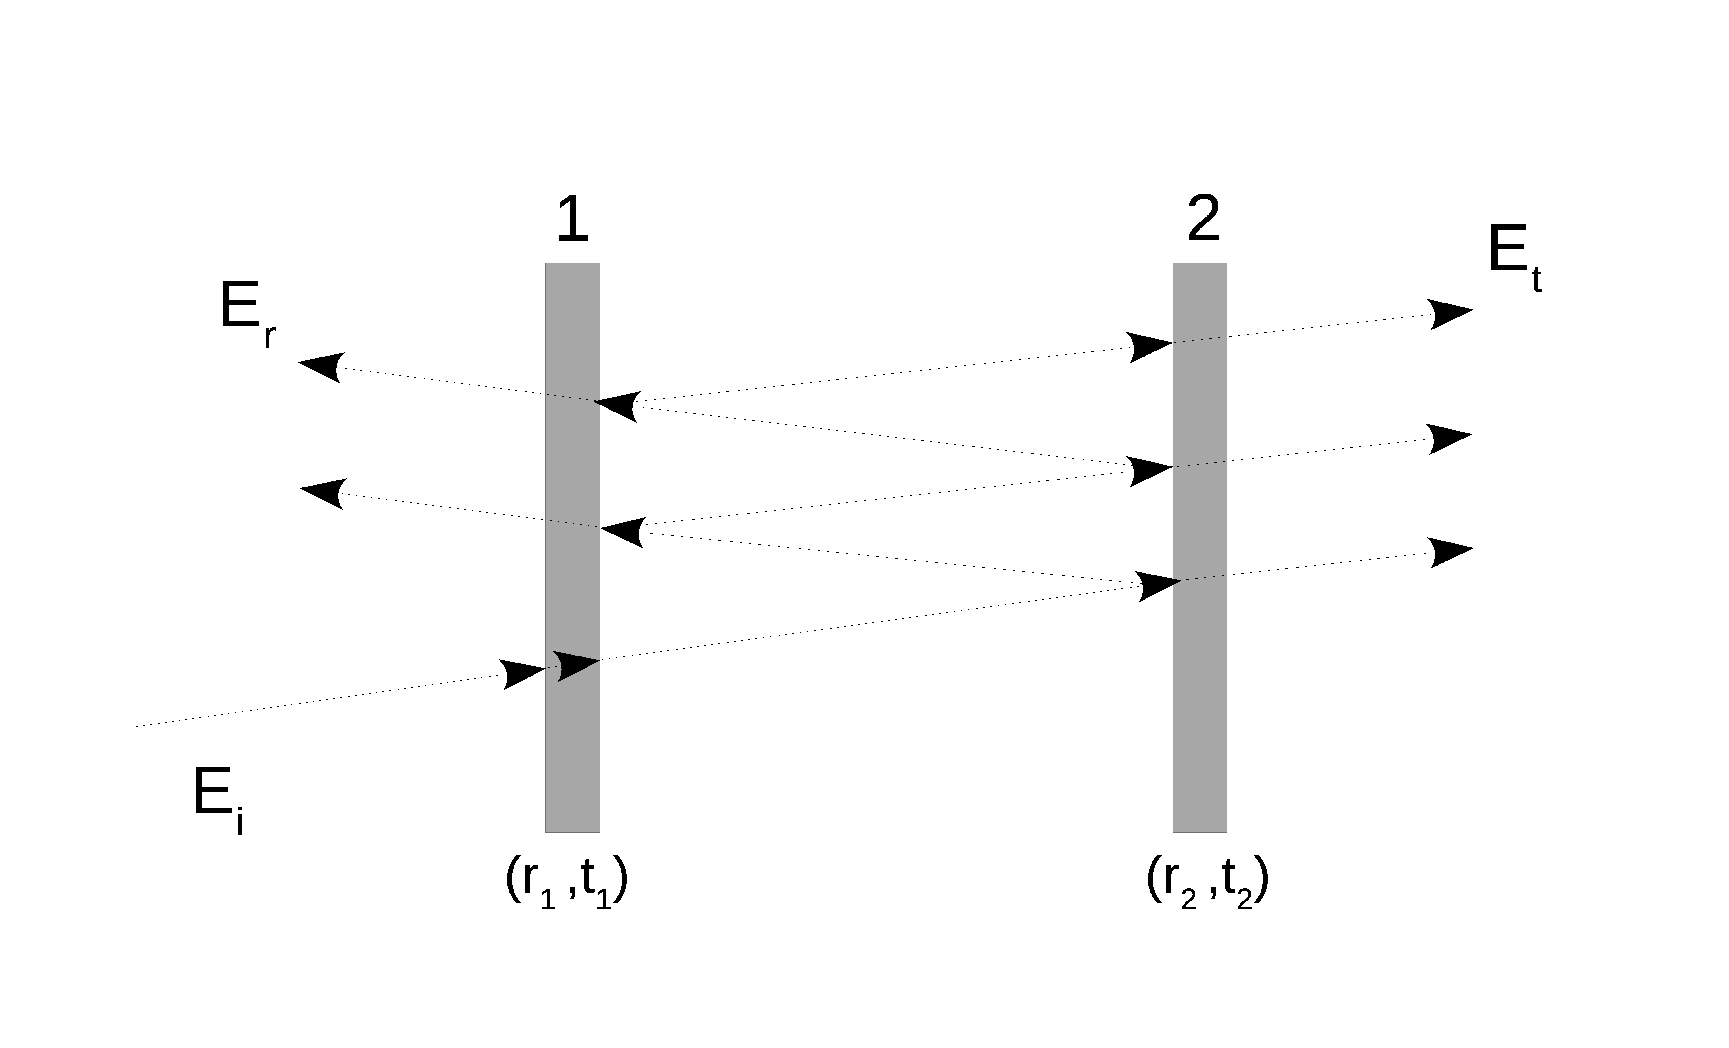
\includegraphics[width=0.60\textwidth]{Fabry_Perot_resonator.eps}
\caption{Illustrated energy diagram of a simple Fabry-Perot resonator}
\end{figure}



\newpage

\subsection{Theory of Fabry-Perot interferometer}
 If the incident energy is in the form of white coherent light then at that point the transmission and reflection coefficients depend just on the mirror reflectivities. The total reflected power comprises of the power reflected from the principal mirror in addition to all the different reflections between the mirrors that add to the reflectivity in general. In summation, the equations are[1]: 
\begin{equation}
{\mathcal R} = R_{1} + T_{1}^2 R_{2} \sum_{m=1}^{\infty} (R_{1}R_{2})^{m-1} = \frac{R_{1} - 2R_{1}R_{2} + R_{2}}{1 - R_{1}R_{2}} _{\overrightarrow{R_{1} = R_{2} \equiv R}} \frac{2R}{1+R}
\end{equation}

Similarly, the transmitted energy in summation is:
\begin{equation}
{\mathcal T} = T_{1} T_{2} \sum_{m=1}^{\infty} (R_{1}R_{2})^{m-1} = \frac{T_{1} T_{2}}{1 - R_{1}R_{2}} _{\; \overrightarrow{R_{1} = R_{2} \equiv R}} \; \frac{T^{2}}{1-R^{2}} = \frac{1-R}{1+R}
\end{equation}

Assuming, be that as it may, the incident light comprises of a transiently lucid (monochromatic) plane wave, at that point the reflected power will be relative to the square of the reasonable total of every reflected field. Since the fields convey phase information with amplitudes added, the division of reflected and transmitted light depends not just on the mirror reflectivities, but in addition on the mirror separation and excitation wavelength. The rational total of fields is amplified when every one of the fields interfere constructively (in phase) and limited when they interfere destructively (out of phase). Phase gathers with propogation separation as $\phi(z) = \beta z$ and may likewise be gained upon communication with the mirrors. The sound forms of 

Eqs. 2.1 and 2.2 incorporate an aggregated stage factor for each round-trip that can be translated as a standardized detuning $\phi = T_{R}\omega$, where $T_{R}$ is the cavity travel time, $T_{R} = n_{eff}L/c$ for the circumference, L and effective index $n_{eff}$. Presently, $\tilde{r}$ speaks to the complex reflectivity:

\begin{multline}
\tilde{r} = r_{1} - t_{1}^{2}r_{2}\exp{(i m \phi)} \sum_{m=1}^{\infty} (r_{1}r_{2}\exp{(i m \phi)})^{m-1} \\ = \frac{r_{1} - r_{2}\exp{(i \phi)}}{1 - r_{1}r_{2}\exp{(i \phi)}} _{\; \overrightarrow{r_{1} = r_{2} \equiv r}} \; \frac{r(1-\exp{(+i \phi)})}{1-r^{2}\exp{(+i \phi)}}
\end{multline}

and $\tilde{t}$ represents the complex transmittivity:

\begin{multline}
\tilde{t} = -t_{1}t_{2}\exp{(i m \phi/2)} \sum_{m=1}^{\infty} (r_{1}r_{2}\exp{(i m \phi)})^{m-1} \\ = \frac{-t_{1}t_{2}\exp{(i m \phi/2)}}{1 - r_{1}r_{2}} _{\; \overrightarrow{r_{1} = r_{2} \equiv r}} \; \frac{-(1-r^{2})\exp{(im \phi/2)}}{1-r^{2}}
\end{multline}


The square modulus of these perplexing amounts gives the reflection ${\mathcal R}$ and transmission ${\mathcal T}$ coefficients (showin in Fig. 2.2). Antiresonant wavelengths are more emphatically reflected than in the ambiguous case, while thunderous wavelengths are transmitted $100\%$ for adjusted reflectors ($r_{1}$ = $r_{2}$). For a fixed reflect dispersing, the transmission and reflection spectra in this manner show intermittent pinnacles and valleys. Figure 2.2 presenting the transmission and reflection spectra for a lossless, adjusted Fabry– Perot resonator. The part of reflected and transmitted power for mixed up excitation is identical to the separate frightfully arrived at the midpoint of reflection and transmission over a time of the spectrum range.

The values of reflectivity coefficients $r_{1}$, $r_{2}$ and the transmitivity coefficients $t_{1}$, $t_{2}$ are mentioned in the figure. The plot is of intensity of the Fabry- Perot resonator versus the round trip phase of the system. This displays a $100\%$ transmission and $0\%$ reflection on the resonant frequencies. Meaning all the incident light is detected on the other side of the resonantor of these specific frequencies. 

\begin{figure}[h]
\centering
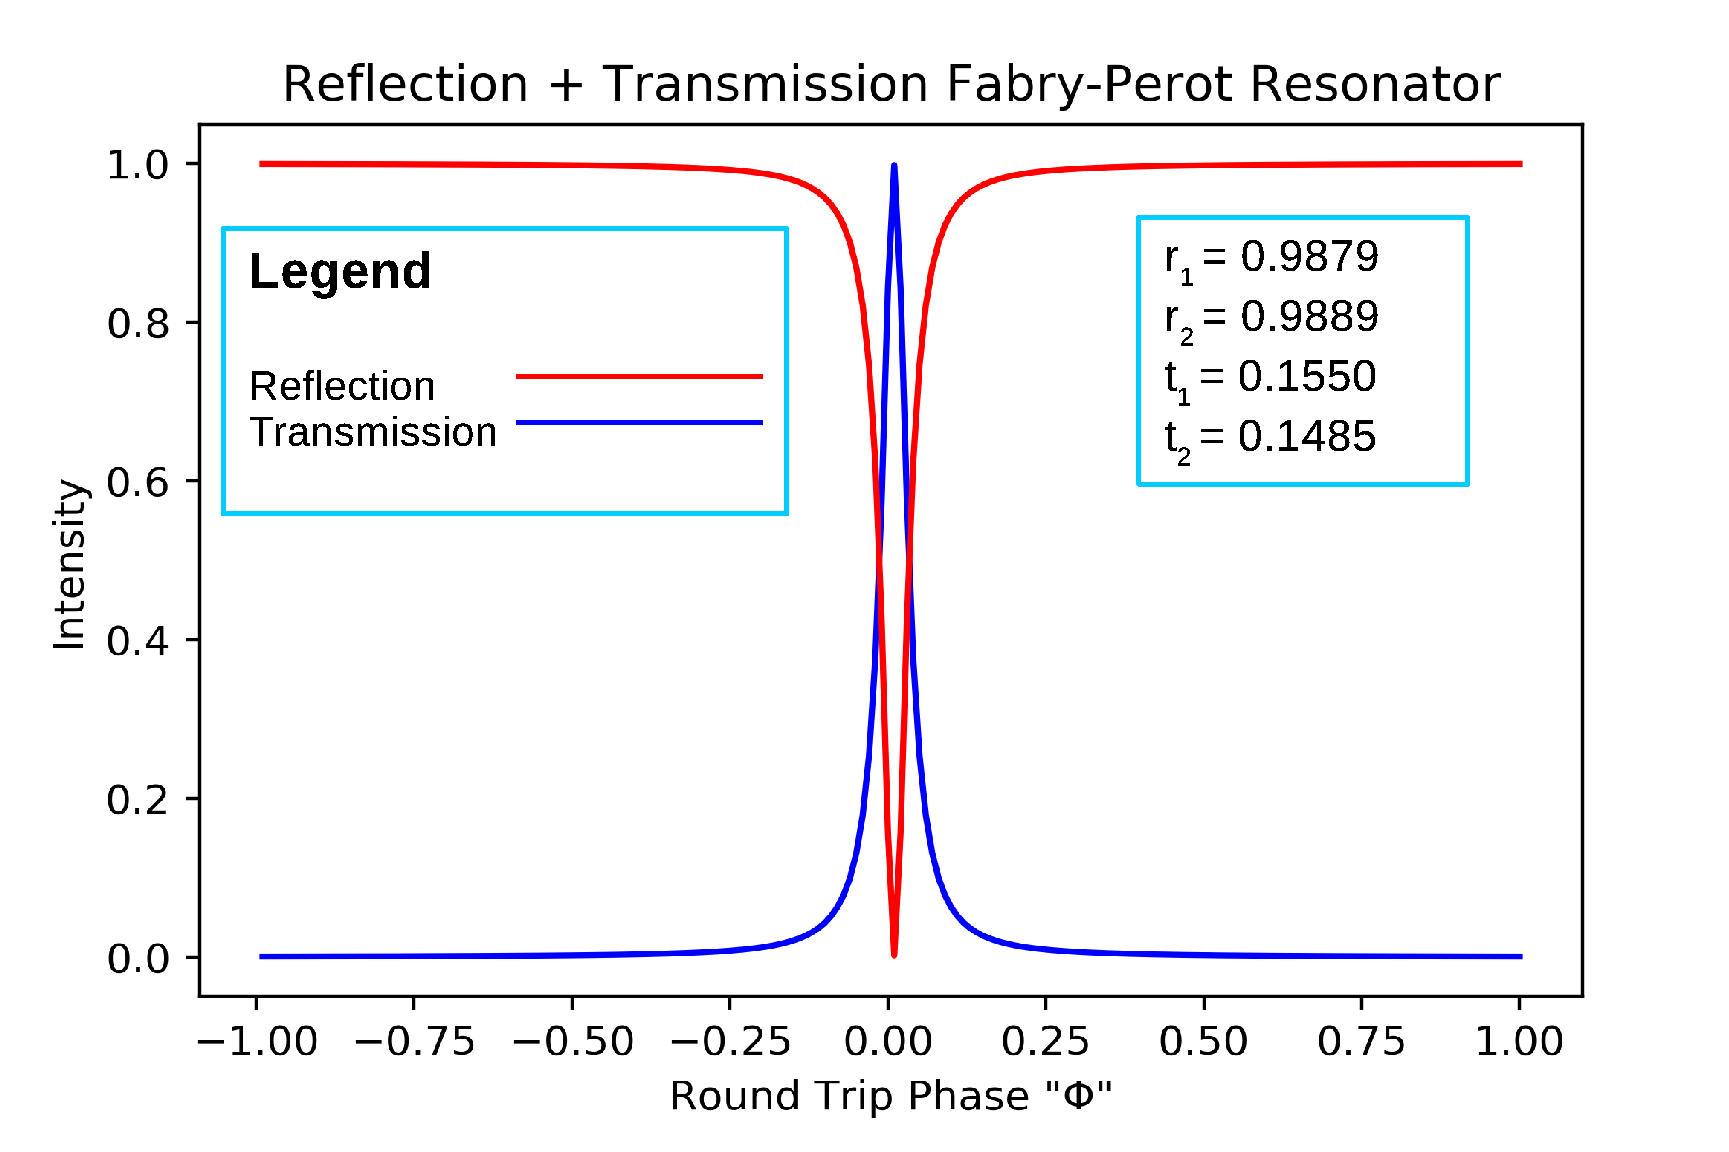
\includegraphics[width=0.85\textwidth]{R+T_FabryPerot.eps}
\caption{Transmitted and reflected field of an asymmetric Fabry-Perot resonator}
\end{figure}

\newpage

\subsection{Effective Phase}
Now lets look at the phase details of the transmission and the refelction spectra of the asymmetric Fabry-Perot resonator. The phase gives us a lot of details about the travelling light inside the resonator and give other details about dispersion, group delay and group index. Fig. 2.3 shows phases of both transmission and reflection of an asymmetric Fabry-Perot resonator.

\begin{figure}[h]
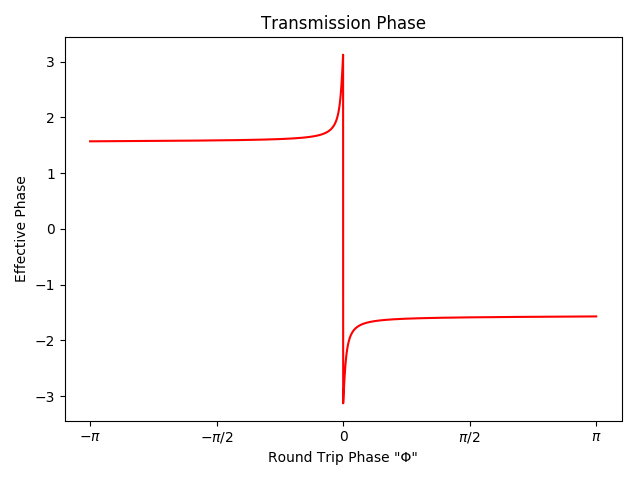
\includegraphics[width=0.5\textwidth]{Phase_trans_FP.png}
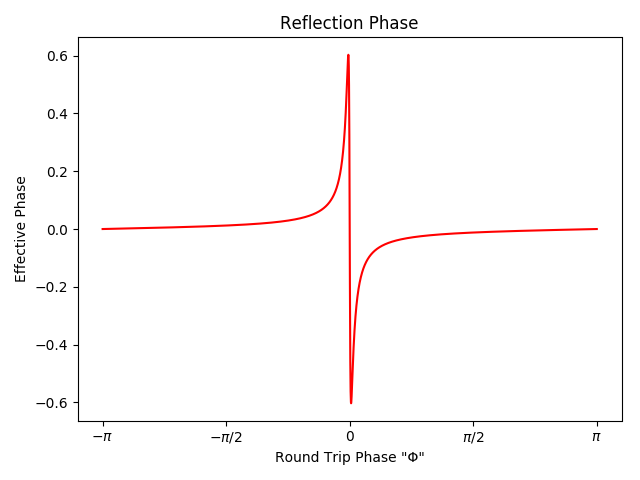
\includegraphics[width=0.5\textwidth]{Reflec_Phase_FP.png}
\caption{Transmission and Reflection phase vs normalized detuning of an asymmetric Fabry-Perot resonator critically coupled.}
\end{figure}

\subsection{Phasor plots}
Phaser plots are another useful way to study the behavior of light inside the optical cavity. The phaser plots are the complex plots between Real and Imaginary parts of the complex reflectivity and transmitivty (equation 2.3 and 2.4 respectively). Figure 2.4 shows the phaser plots of both transmitivity and reflectivity of an asymmetric Fabry-Perot resonator over the detuning period of 0 to $2\pi$ radians. 

\begin{figure}[h]
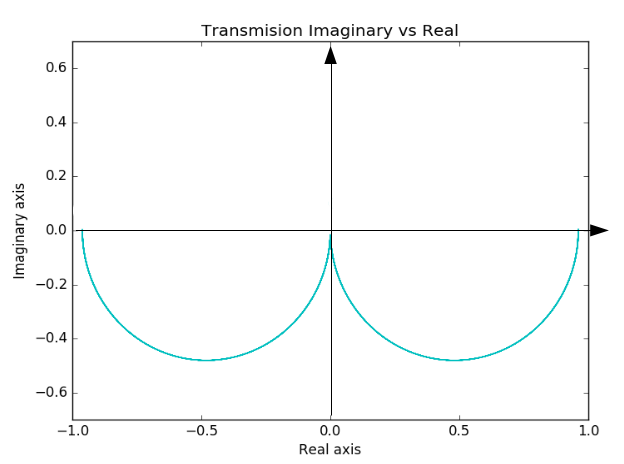
\includegraphics[width=0.5\textwidth]{Trans_ImagvsReal_Phaser.png}
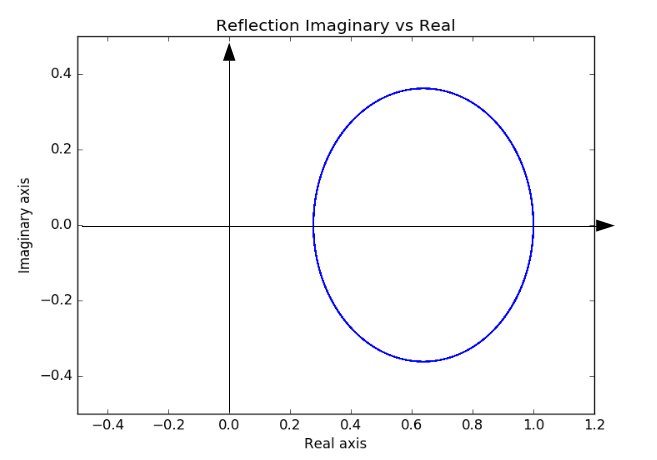
\includegraphics[width=0.5\textwidth]{Reflection_ImagvsReal_Phaser.png}
\caption{Phaser plots of complex Transmitivity and Reflectivity of an asymmetric Fabry-Perot resonator from 0 to $2\pi$}
\end{figure}

\subsection{Finese, Q-factor}
\subparagraph{\normalfont \large The resonance condition is fulfilled when the (compelling) circumference of the ring, or for the most part the round-trip length, is equivalent to a whole number numerous of the optical wavelength inside the medium. This means a progression of Lorentzian-molded transmission bends equally dispersed in recurrence by the FSR (Free Spectral Range), with the resonance linewidth portraying the capacity time of photons inside the cavity. The photon 	lifetime can be standardized to one optical cycle, known as the quality factor (${\mathcal Q}$), or the cavity round-trip time, known as the cavity Finesse (${\mathcal F}$). The most extreme reachable Q-factor is characterized as ${\mathcal Q_{int}}$, which is the intrinsic loss of the cavity. At the point when the resonator is coupled to the outer world, the Q-factor further decreases because of the loss imported by the coupler (${\mathcal Q_{ext}}$). Thus the last quality factor ${\mathcal Q_{load}}$ is comprised of these two parts: ${\mathcal Q_{load}^{-1}}$ = ${\mathcal Q_{int}^{-1}}$ + ${\mathcal Q_{ext}^{-1}}$.}

\begin{align*}
{\mathcal F}inese = \frac{FSR}{FWHM} \\ 
\\
{\mathcal F}inese = \frac{2\pi}{2ra\cos{(\frac{2ra}{1+a^{2}r^{2}})}} \\
\end{align*}
{\normalfont If $ra = 1$ then,} \\
\begin{equation}
{\mathcal F}inese = \frac{\pi}{1-ra}
\end{equation}

Similarly, 

\begin{align*}
{\mathcal Q}_{factor} = \frac{\lambda_{res}}{FWHM} \\ 
\\
{\mathcal Q}_{factor} = \frac{nLf}{\lambda} \\
\end{align*}
\begin{equation}
{\mathcal Q}_{factor} = m f
\end{equation}


\section{Gain incorporation in Resonators}
Light, when travels through a medium, loses its intensity exponentially. This law is called the $Beer's law$ for electromagnetic intensity. But some mediums, whose refractive index is such as they oppose the exponential decay of the light and rather increase the intensity in the propogation through the medium, are called natural gain medium. Also, there can be artificial source to activate gain in a certain system. This is done by pumping energy or external light source i-e. Lasers, to excite the atoms inside the cavity. This makes the stimulated emmission releases of the photons increase exponentially and we see increase in the incident intensity of the input light. We can use these gain mediums and build microresonators from them and observe different quantum optical phenomenons. First I will explain a bit about how gain works.


\subsection{Beer's Law}
The simple radiation law follows the beer's law in absorption of any kind of radiation inside a medium. This tells us that the initially intensity of the light source depends on the variables of the medium it is passing through. For electromagnetic radiation, we can write this law as,

\begin{equation}
I(z) = I_{o}\exp(-\alpha z)
\end{equation}

Here, $I_{o}$ is the initial intensity of the radiation, $\alpha$ is the attenuation constant of the medium, $z$ is the amount of distance traveled through the medium and $I(z)$ is the intensity of light after traveling the distance $z$.

\begin{figure}[h]
\centering
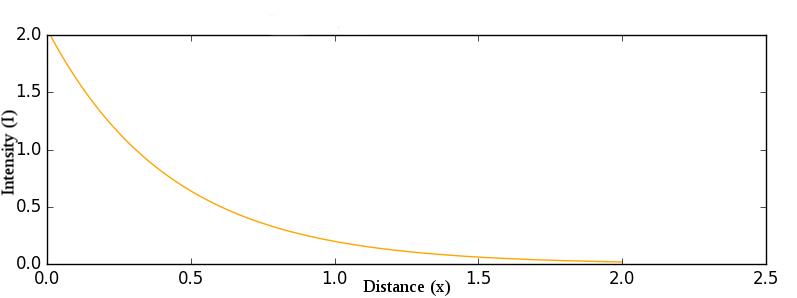
\includegraphics[scale=0.75]{beer's_law_withoutgain.png}
\caption{Beer's law plot with attenuation 0.01/cm: y-axis shows the intensity of light and x-axis shows the distance traveled in meters.}
\end{figure}


\subsection{Beer's law study as gain}
In a gain medium, the intensity of the light will not decrease but it will gradually increase. This means that the attenuation $\alpha$ is negative or we can introduce a new coefficient for such medium say $g$ such that $-\alpha \to +g$ where $g$ is some positive real number. This means that the intensity function now grows exponentially rather than decaying exponential.

\begin{equation}
I(z) = I_{o}\exp( +g z)
\end{equation}

\begin{figure}[h]
\centering
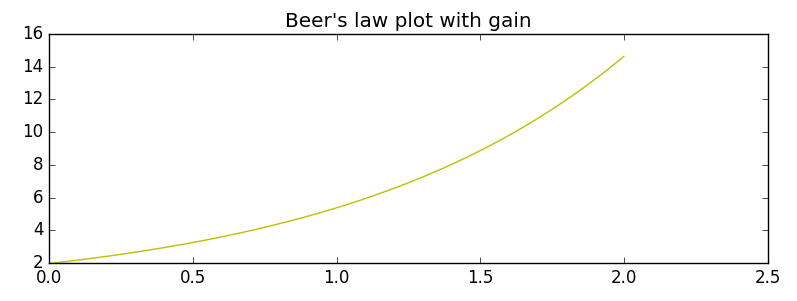
\includegraphics[scale=0.75]{beer's_law_withgain.png}
\caption{Beer's law plot with gain value 0.01/cm: y-axis shows the intensity of light and x-axis shows the distance traveled in meters.}
\end{figure}

\subsection{Gain medium}
The active laser medium also called gain medium or lasing medium is the source of optical increase inside a laser. The gain is the result of stimulated emmision of electronic or sub-atomic changes to a lower energy state from a higher energy state recently populated by a pump source. This gain in optical systems is usually used for amplification purposes and hence make optical amplifiers.


\section{Ring Geometry Resonators}
In this section, I will discuss different kinds of ring shaped resonators whose principle is pretty much similar to the Fabry-Perot resonator and are more simple to make. Basically, a ring resonator is a simple waveguide which is turned in the shape of a ring. This allows it to exhibit resonant behavior on very specific frequencies. The light is coupled inside the ring due to the phenomenon of total internal reflection and interference. This kind of behaviour is noticed in all kind of classical waves, such as sound waves, which was observed inside a large cathedral's halls, thus it was named whispering galleries. Also, these resonators can be made using different material but in this thesis, we used semi-conductor silicon as the primary material. 

\subsection{Evanescent Coupling}
This optical system experiences passage of light through both of the rings through evanescent coupling, a classical phenomenon with quantum like properties. This evanescent coupling allow the light propagation through the both rings of the resonator making it a composite of resonant wavelength systems. This is the power transfer of the wave which is dependant on the proximity of the optical resonator and the waveguide also the length or area that has been exposed to the coupler also plays an important role i-e how much part of the waveguide/resonator overlaps; shown in Fig. 2.17.
\subparagraph{\normalfont \large Coupling strength of an ideal coupler is dependant on the interaction length between the two optical modes which means power will transfer more efficiently when the two modes are mathced on the basis of their respective phases.  This allow us to observe distinct behaviors as well as multiple resonances in transmittance and reflectance.} 

\begin{figure}[h]
\centering
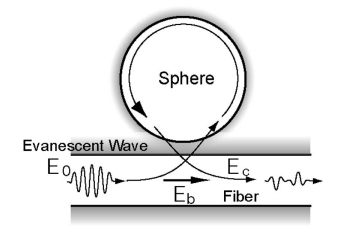
\includegraphics[width=0.50\textwidth]{evanescent_wave.png}
\caption{Schematic illustration of the microsphere-fiber-taper
system.[2]}
\end{figure}

\section{Coupling Regimes}
here I will discuss different coupling regimes for these resonators. plots are done for all pass resonator for under over and critically coupled system as well as the system in which r1 = r2 = 1 where all the light is transmitted from the all pass resonator. the graph shows pink for critical, red for over couple and green for under couple. also there is a single transmission line in orange showing 100 percent transmittance.


\begin{figure}[h]
\centering
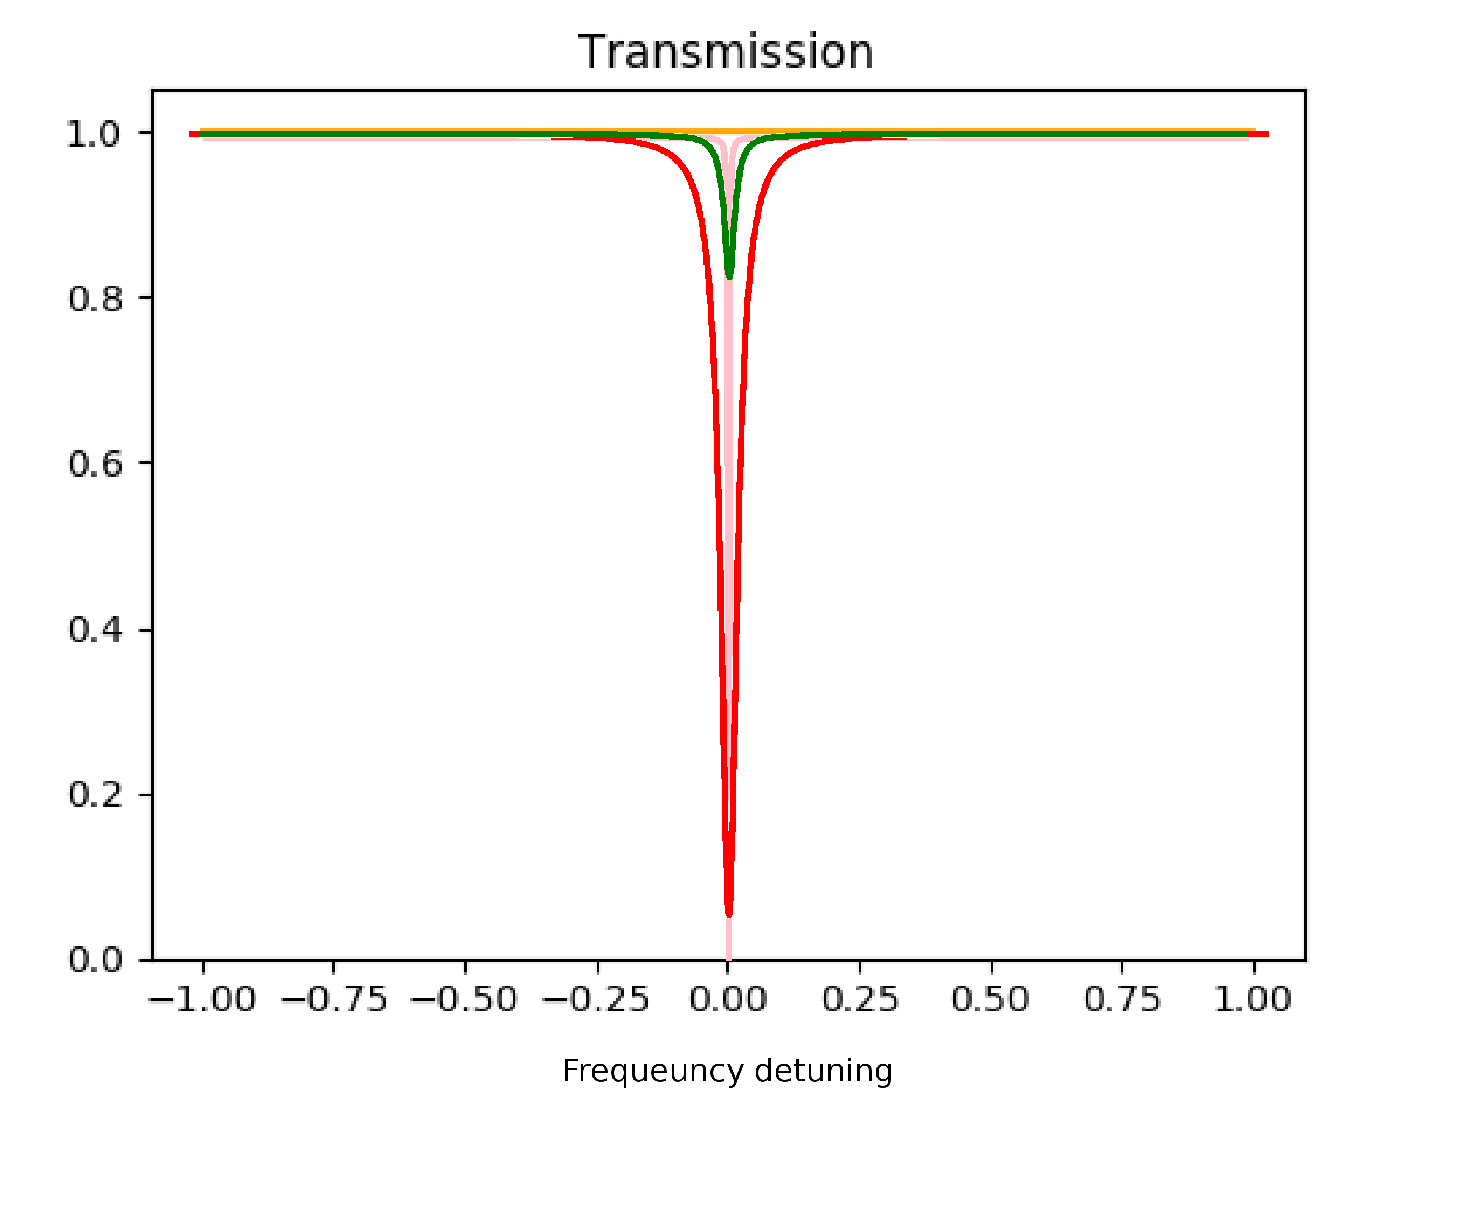
\includegraphics[width=1\textwidth]{under_over_couple.eps}
\caption{different coupling shown in different colors.}
\end{figure}

\subsection{All-Pass Ringresonator}
A straightforward ring resonator is made by taking one yield of a conventional directional coupler and bolstering it once again into one input. Such a device displays periodic cavity resonance (reverberation) when light navigating the ring procures a phase move relating to a number numerous of 2$\pi$ radians. The resonator is numerically defined from two parts: a coupling quality and an input way. In opposition to the limitless entirety inferences performed before for the Fabry– Perot and Gires– Tournois, in which we expected steadystate task and coordinating fields and derived basic spectral properties. Although, both strategies are similarly substantial, the field-coordinating technique has the benefit of simplicity.
\begin{figure}[h]
\centering
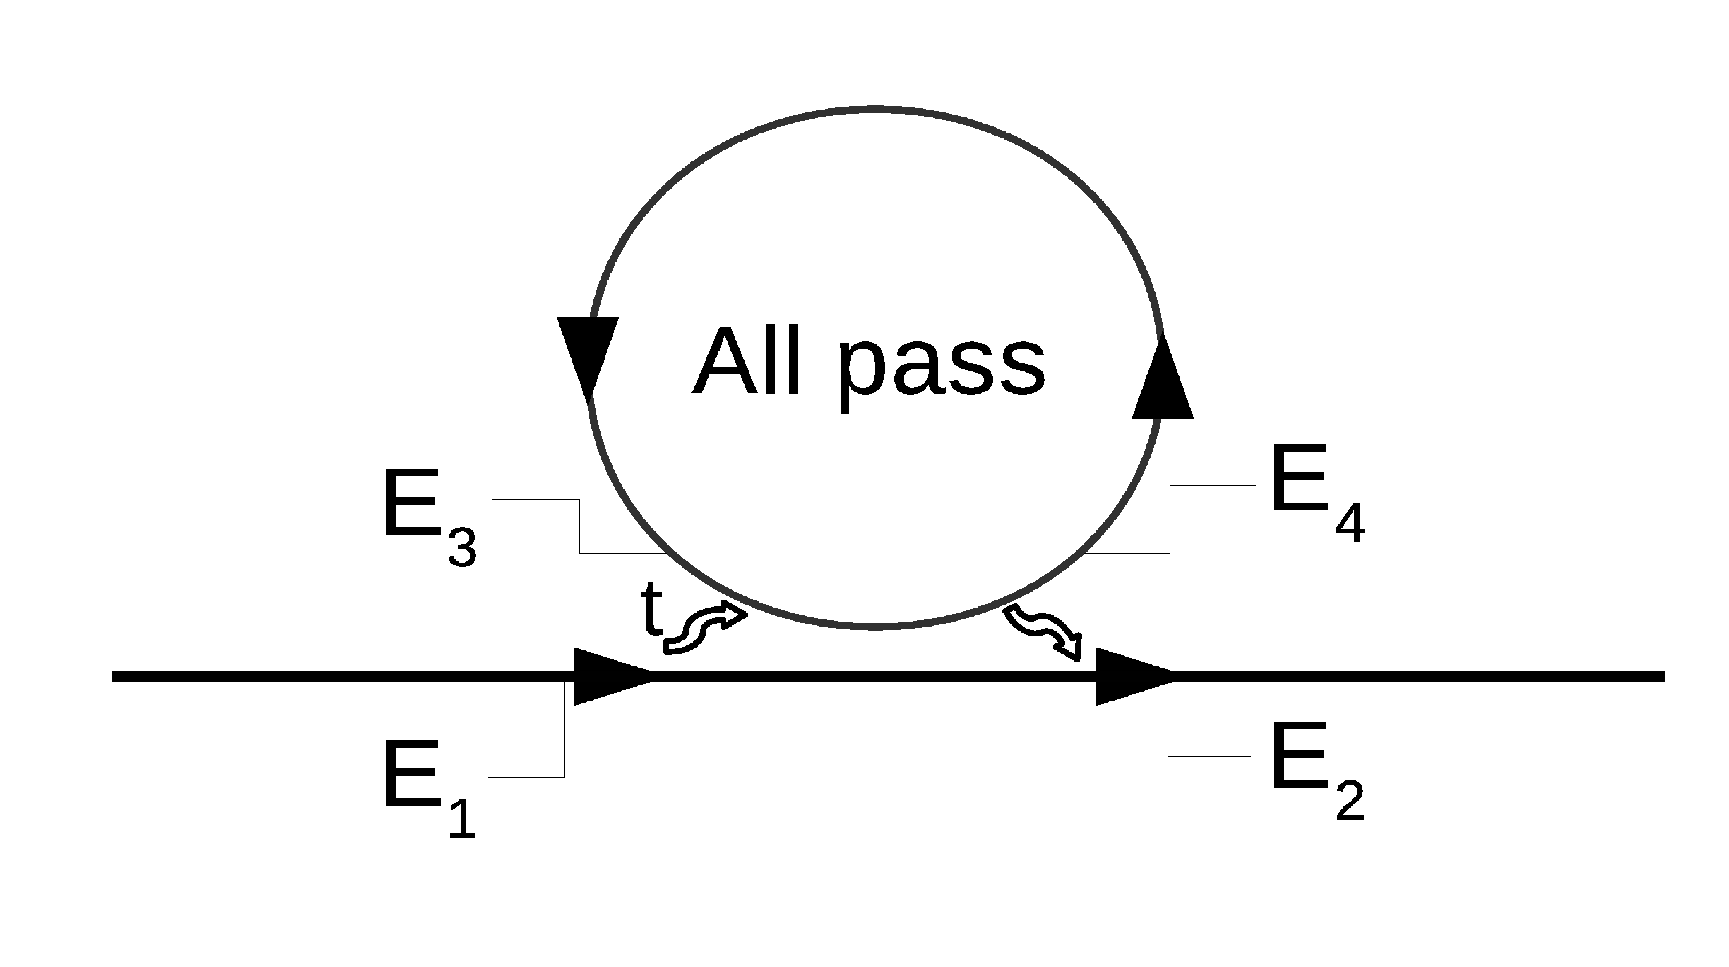
\includegraphics[width=0.85\textwidth]{all_pass_resonator.eps}
\caption{Illustrated fields of an all pass resonator}
\end{figure}

Fig. 2.8 illustrates the basic geometry of the all-pass ring resonator. The complex transmitivity and reflectivity is given by equation 2.9 and 2.10 respectively.

\begin{equation}
\frac{E_{t}}{E_{i}} = \frac{r_{1} - a_{1} e^{i\phi_{1}}}{1 - r_{1} a_{1} e^{i\phi_{1}}}
\end{equation}

\begin{equation}
\frac{E_{r}}{E_{i}} = \frac{- t_{1} t_{2} a_{1} e^{i \frac{\phi_{1}}{2}}}{1 - r_{1} a_{1} e^{i\phi_{1}}}
\end{equation}

\subsubsection{Transmission and Reflection}
Let us now look at some reflection and transmission spectra of a passive All-pass ring resonator. Fig. 2.6 shows that the transmission and reflection peaks are flipped as in case of an symmetric Fabry-Perot resonator.
\begin{figure}[h]
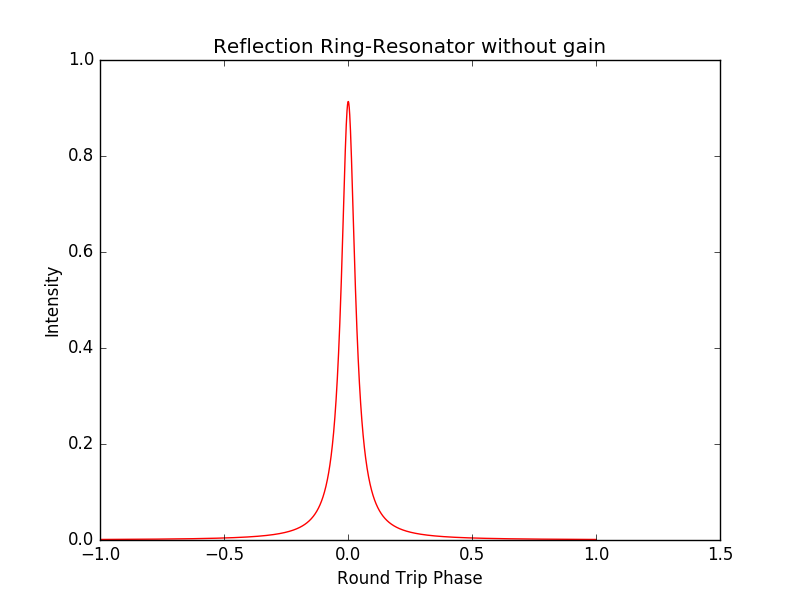
\includegraphics[width=0.5\textwidth]{reflec_ring_withoutgain.png}
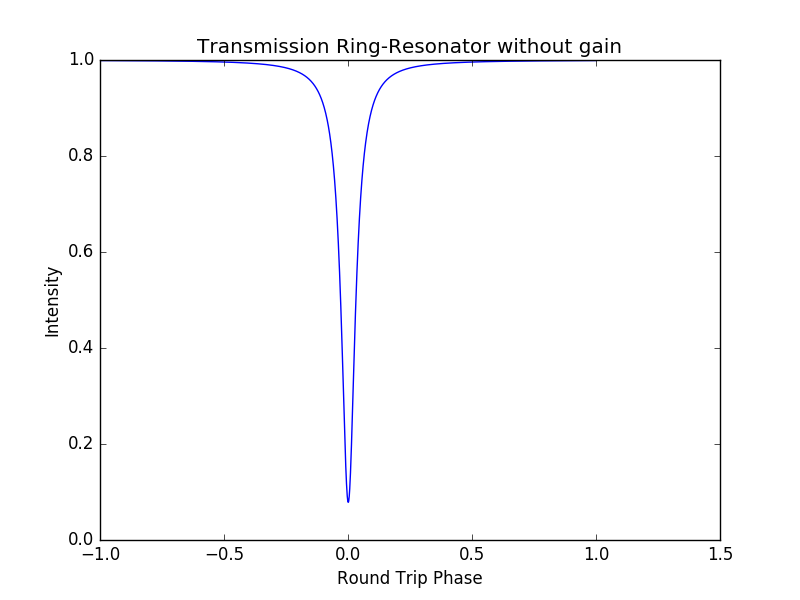
\includegraphics[width=0.5\textwidth]{trans_ring_withoutgain.png}
\caption{Reflection and Transmission spectra of a passive All-pass ring resonator}
\end{figure}

\subsubsection{Transmission and Reflection with gain}
Now we introduce gain into the system and observe that the tranmission dip also shifts into a peak and go way above the 1 mark meaning that it is greater than the initial intensity and the reflection peak is also above 1 mark meaning a lot of incident light is being reflected. We will study the transmission of some other different geometries of ring resonators with gain. 

\begin{figure}[h]
\centering
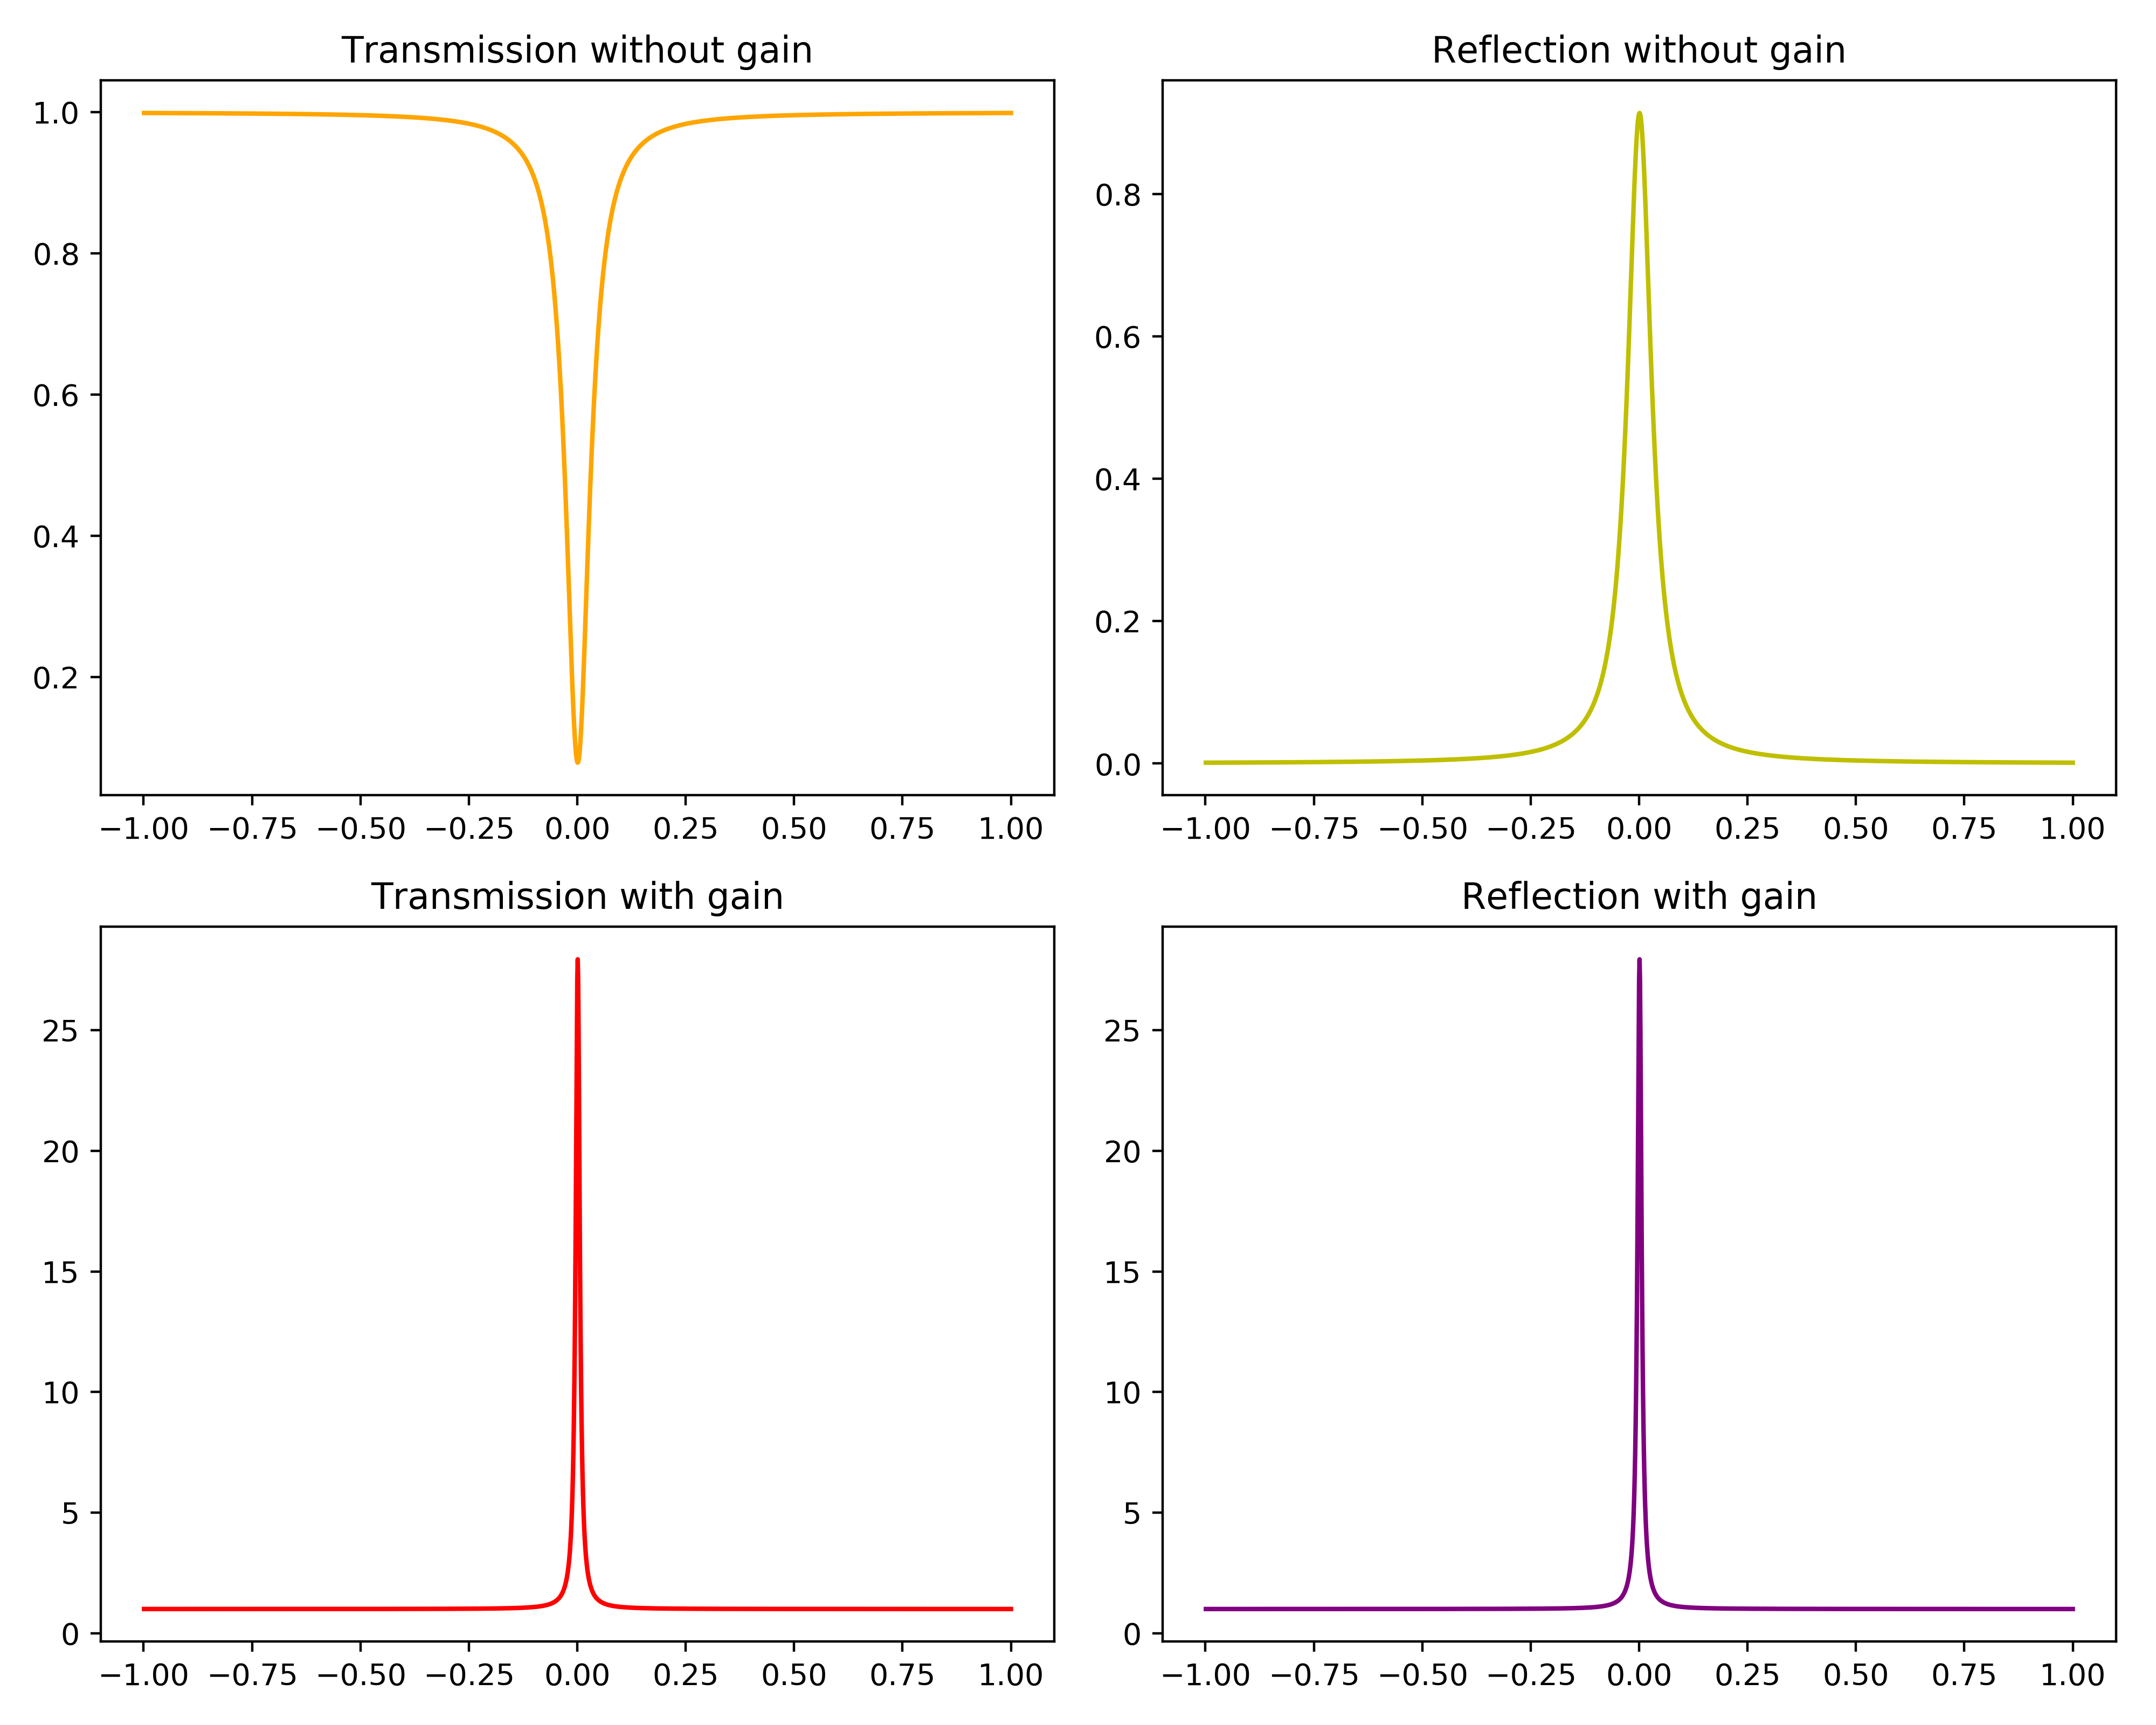
\includegraphics[width=0.80\textwidth]{all-pall_gain.png}
\caption{Gain introduced into an all-pass resonator: we see clear difference in the intensities.}
\end{figure}


\subsubsection{Effective Phase}
The phase of the All-pass ring resonator is shown in Figure 2.7. We can easily observe from this that with changing the values of the coupling $r$, the shapre of the graph changes as that of a function of $ArcTan\phi$. The relation for phase is given by,
\begin{equation}
\Phi_{eff} = \pi + \phi + 2\tan^{-1}\frac{r\sin\phi}{1-r\cos\phi}
\end{equation}

\begin{figure}[h]
\centering
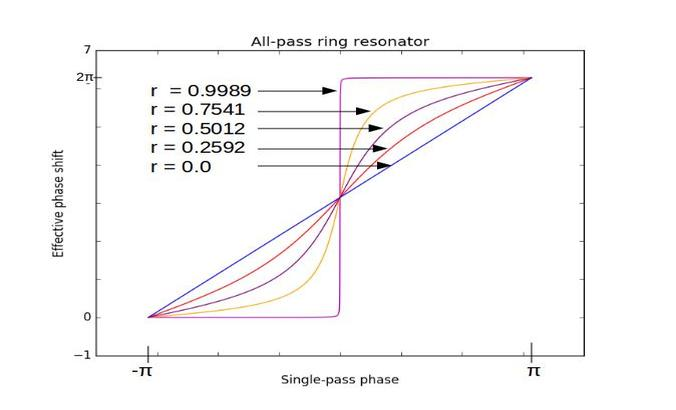
\includegraphics[width=0.65\textwidth]{allpassphase_new.png}
\caption{Phase diagram of an All-Pass ring resonator from 0 to $\pi$ where $r$ is the coupling parameter.}
\end{figure}
\newpage

\subsubsection{Phasor Plots}
Now looking into some complex refractivity and transmitivity of an All-pass ringresonator (Fig. 2.7). These plots are plotted over the complex plain from the detuning limits of 0 to 2$\pi$. The transmission loop does not go to negative real axis and touches the origin but the reflection curve does not even form a loop.
\begin{figure}[h]
\centering
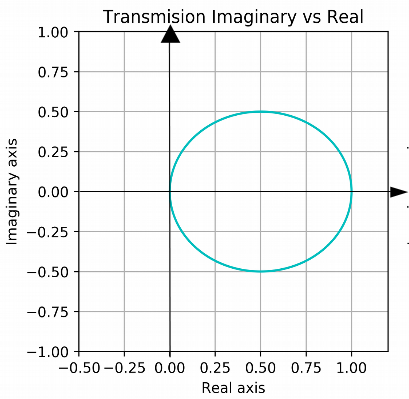
\includegraphics[width=1\textwidth]{Imag_vs_real_allpass.png}
\caption{Phaser plots of complex Transmitivity and Reflectivity of an All-pass ring resonator}
\end{figure}
\newpage

\subsection{Add-Drop Ringresonator}
The immediate waveguide similarity of a free-space Fabry– Perot is gotten by including a second guide that side-couples to the resonator as in Fig. 1.4.
Since this setup acts as a tight band abundancy channel that can include or drop a recurrence band from an approaching sign, it is regularly named as an add– drop filter. Fig. 2.8 shows the basic geometry of the add-drop ring resonator with its associated fields labeled accordingly. This resonator has an input, through and drop interfaces where $t_{1}$ is add and $t_{2}$ is drop coefficients.Input field is labeled as $E_{1}$ while the through field is labeled as $E_{2}$. The drop field is on the left top corner lableled as $E_{5}$. The ratio of these fields to the incident/input field defines the total transmitivity and total reflectivity of the filter. 
\begin{figure}[h]
\centering
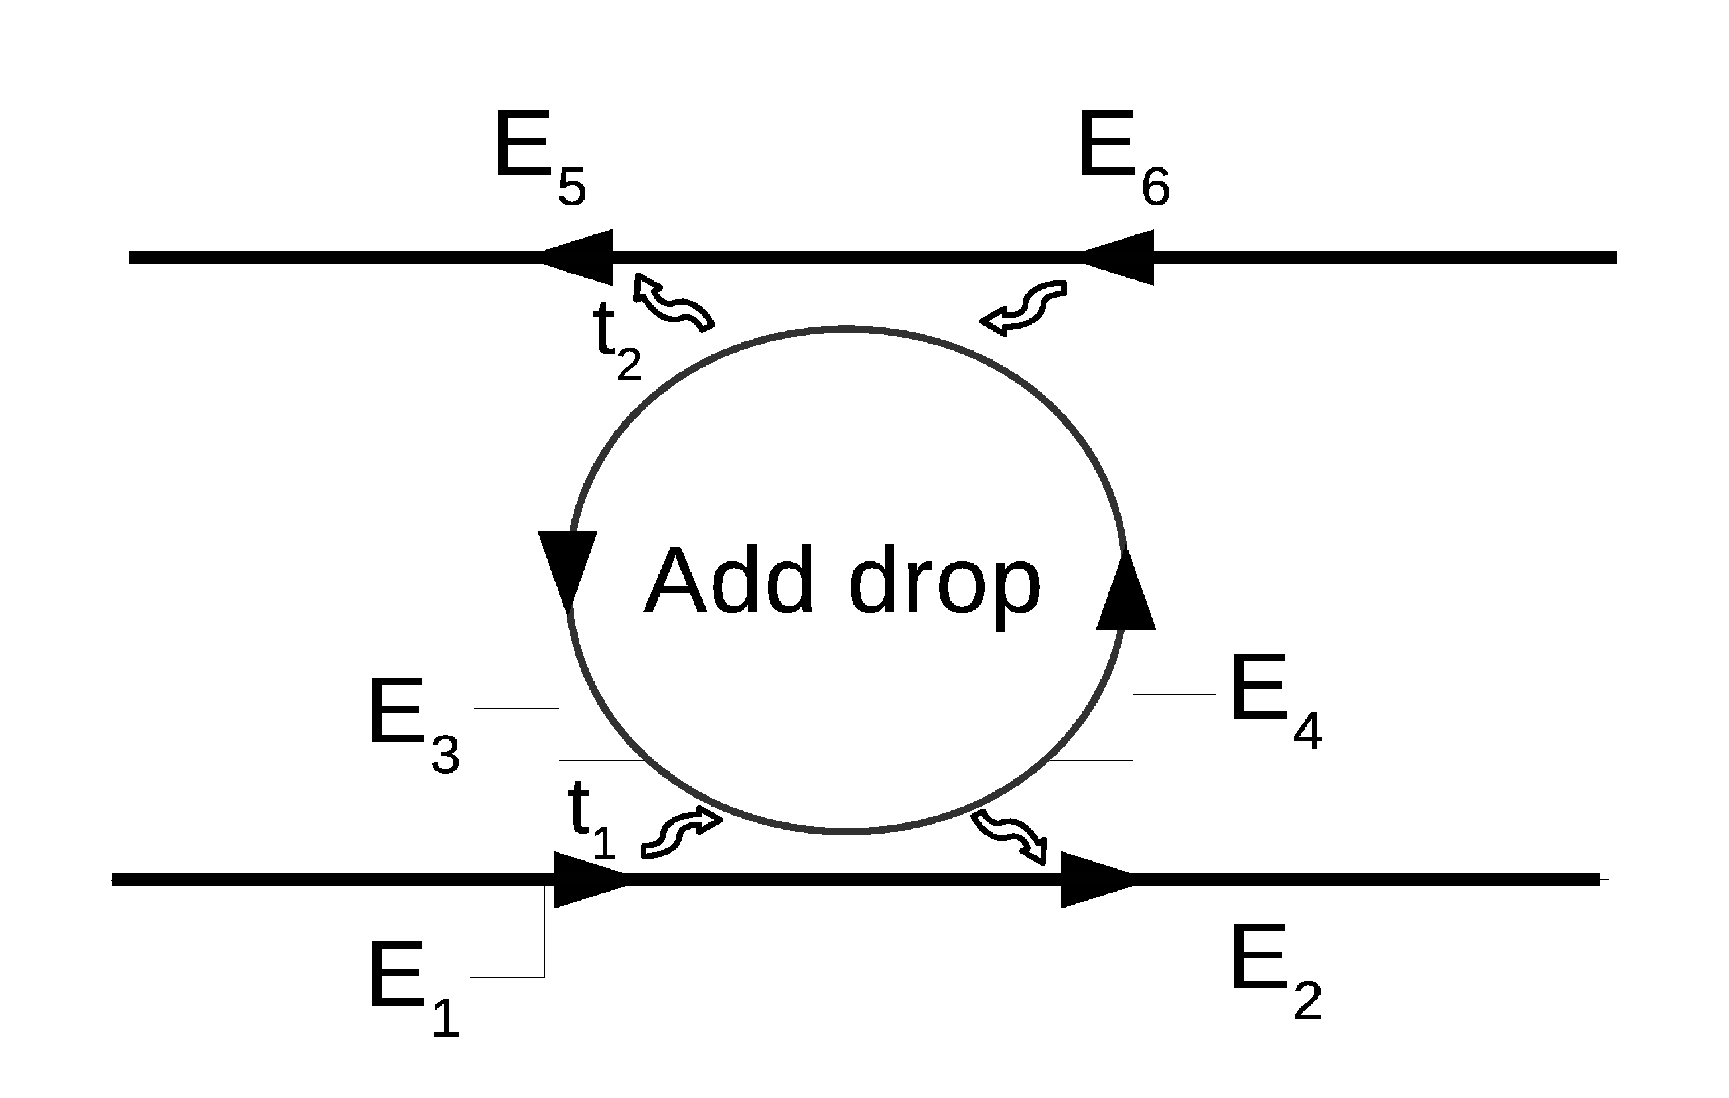
\includegraphics[width=0.70\textwidth]{add_drop_resonator.eps}
\caption{Illustrated fields of an add drop resonator}
\end{figure}

The transmission and reflection relations are given as,

\begin{equation}
\frac{E_{t}}{E_{i}} = \frac{r_{1} - r_{2} a_{1} e^{i\phi_{1}}}{1 - r_{1} r_{2} a_{1} e^{i\phi_{1}}}
\end{equation}

\begin{equation}
\frac{E_{r}}{E_{i}} = \frac{- t_{1} t_{2} a_{1} e^{i \frac{\phi_{1}}{2}}}{1 - r_{1} r_{2} a_{1} e^{i\phi_{1}}}
\end{equation}



\subsubsection{Transmission and Reflection}
Let us now look at some reflection and transmission spectra of a passive Add- drop filter. Fig. 2.10 shows that the transmission and reflection peaks are flipped as in case of an asymmetric Fabry-Perot resonator and the transmission phase is a direct function of the detuning. Reflection phase is also shown in Fig. 2.11.

\begin{figure}[h]
\centering
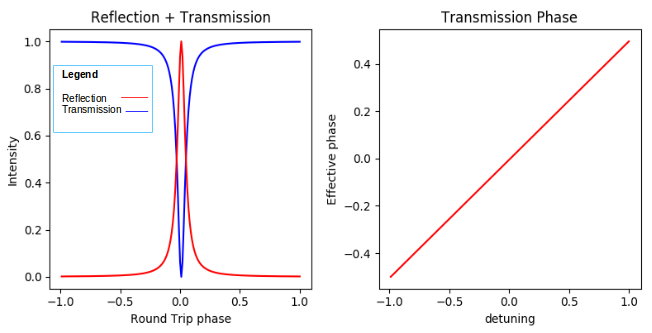
\includegraphics[width=0.85\textwidth]{all_pass_plots_a.png}
\caption{Reflection and Transmission spectra along with transmission phase} 
\end{figure}
\newpage
\begin{figure}[t]
\centering
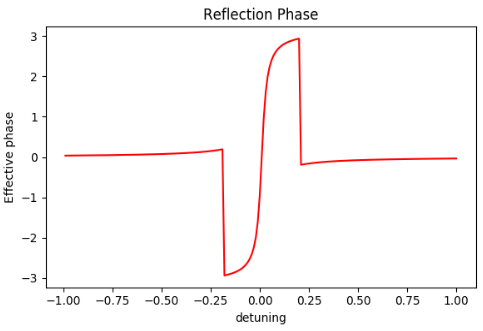
\includegraphics[width=0.5\textwidth]{all_pass_plots_b.png}
\caption{Reflection phase of the all-pass ring resonator.}
\end{figure}

\subsubsection{Transmission and Reflection with gain}
Now we introduce gain into the system and observe that the tranmission dip also shifts into a peak which above the 1 mark meaning that it is greater than the initial intensity and the reflection peak is almost near zero meaning most of the incident light is being transmitted. We will study the transmission of some other different geometries of ring resonators with gain. 


\begin{figure}[h]
\centering
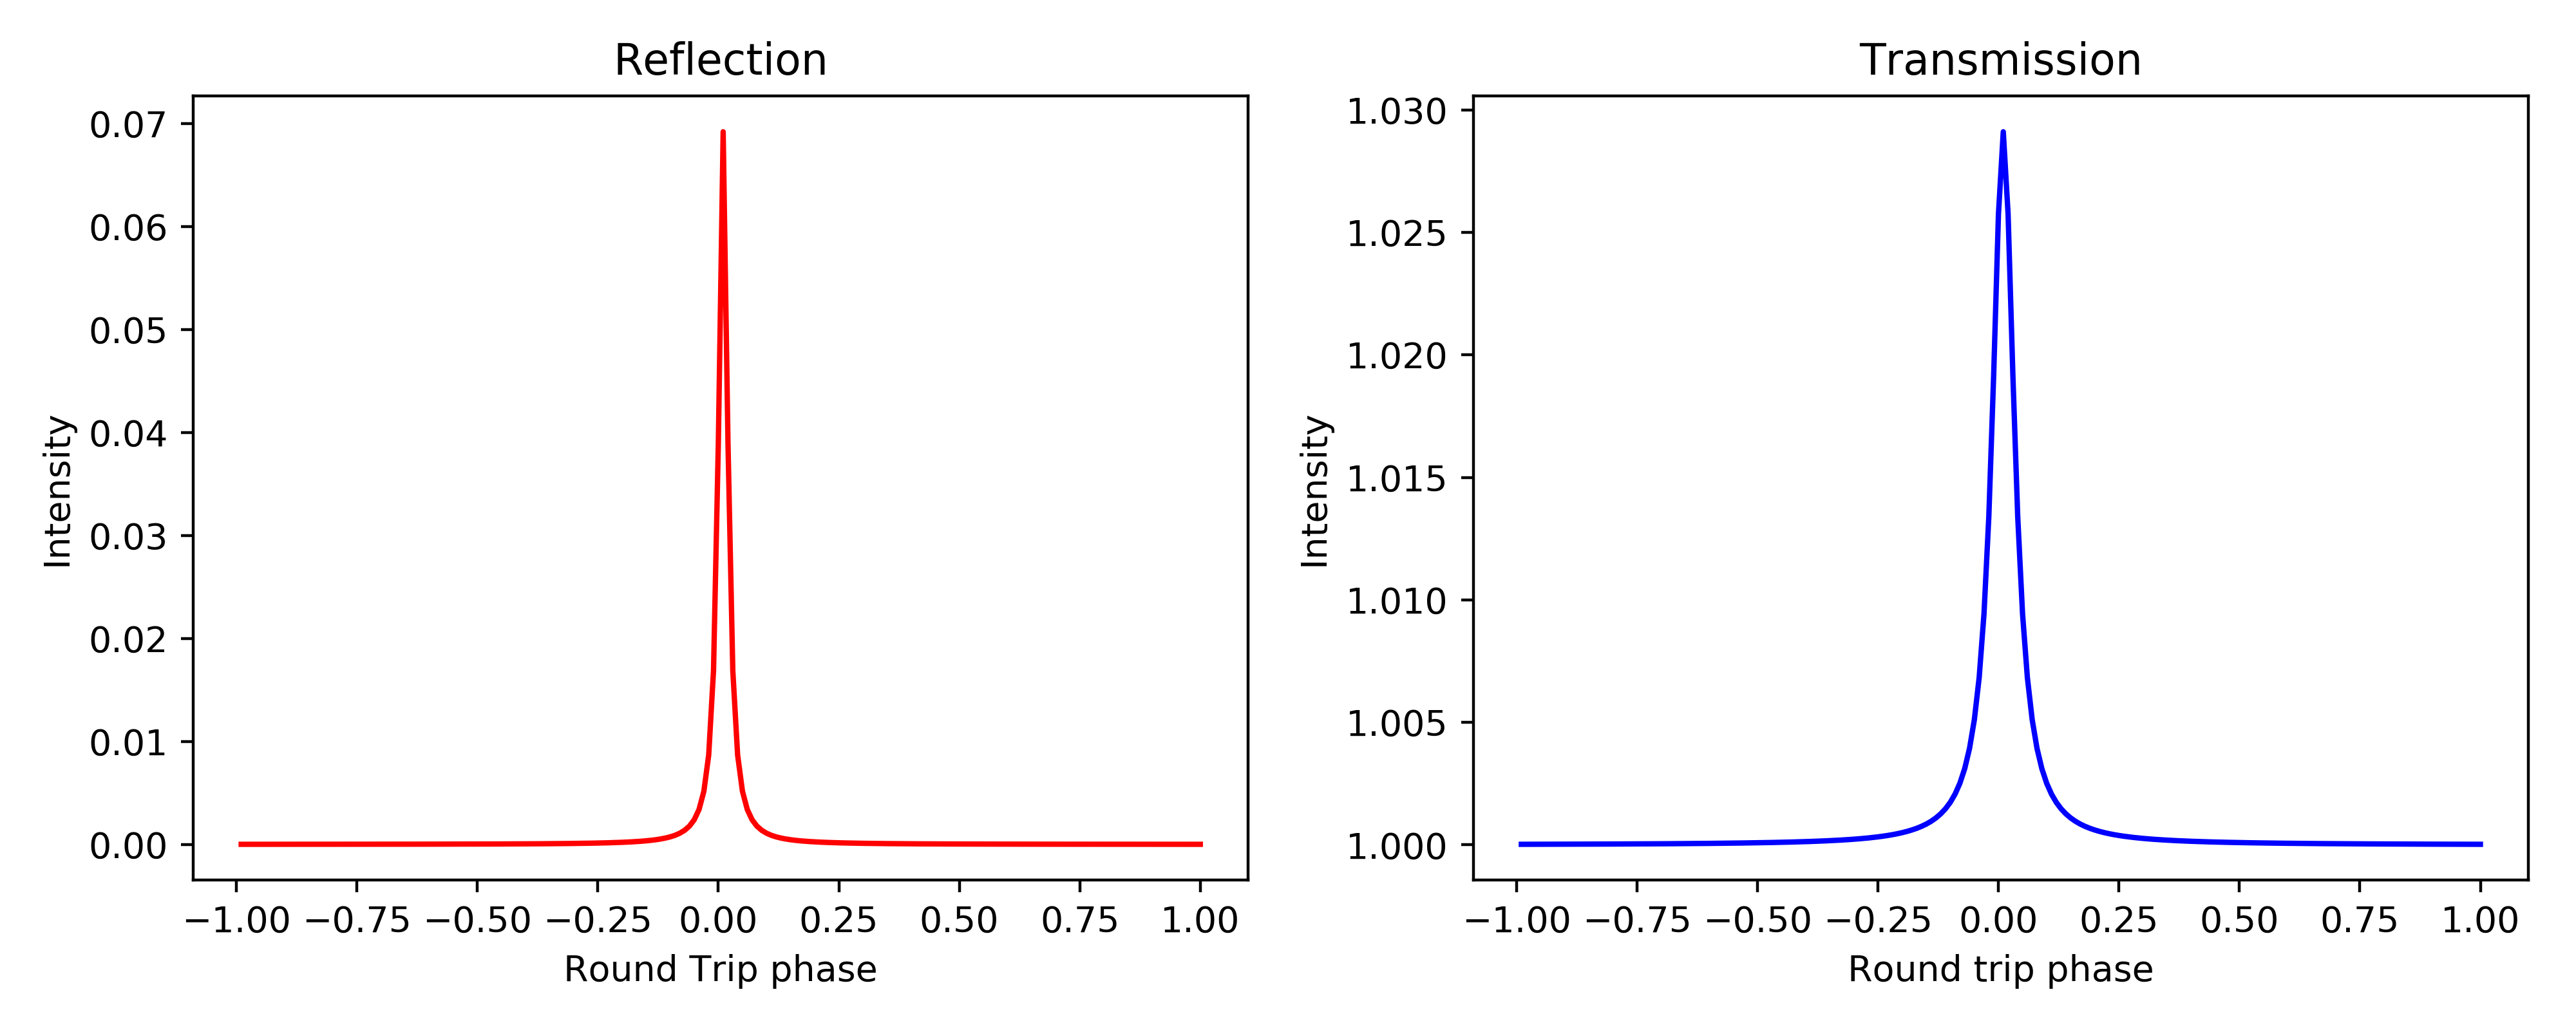
\includegraphics[width=0.85\textwidth]{add_drop_gain_plots.png}
\caption{Gain introduced into an all-pass resonator: we see clear difference in the intensities.}
\end{figure}
\newpage

\subsubsection{Phasor Plots}
Now let us see how complex plots of Add drop is different from the All-pass resonator. Fig. 2.11 shows that the loop goes towards the negative real axis as the phase is increased. This tells a lot about the distinct behavior.

\begin{figure}[h]
\centering
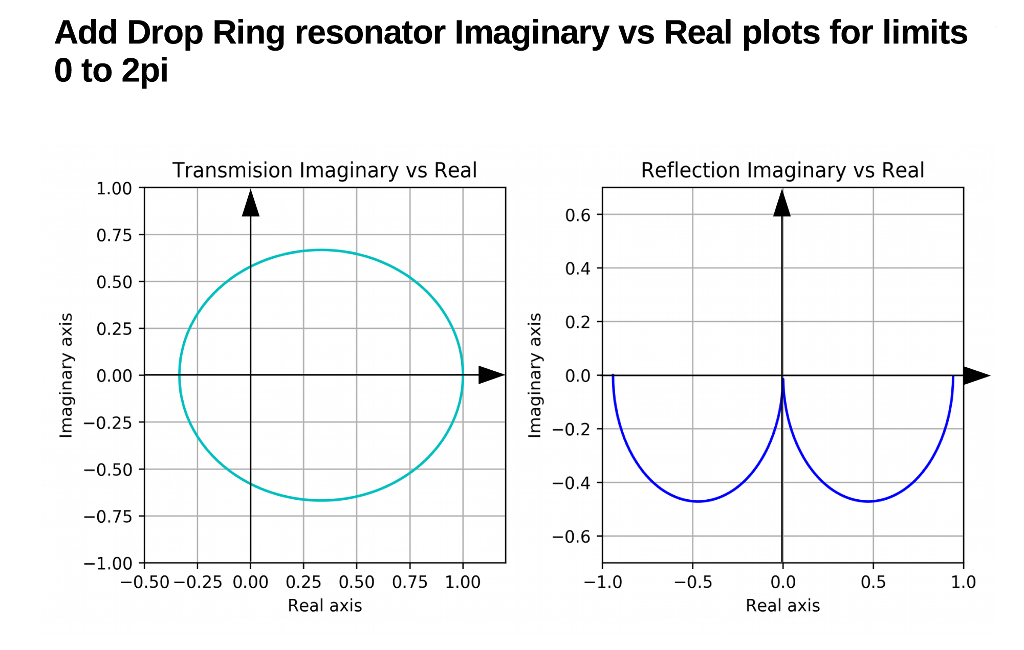
\includegraphics[width=1\textwidth]{ImagVsReal(add-drop).png}
\caption{Phaser plots of complex Transmitivity and Reflectivity of an All-pass ring resonator from 0 to $2\pi$}
\end{figure}
\newpage

\section{Coupled Ring Resonator}
Now we turn another optical waveguide into a ring shape and install it on the top of the all-pass ring resonator such that now we have dual ring geometry and a wave guide coupler. This geometry does allow resonant behaviors and the spectra varies largely from an all-pass resonator.
In this arrangement, coupling between the two resonators (rings) also play an important role in the spectra of the light that passes through the resonator. Fig. 2.16 displays the basic geometry of the couple ring system we are going to discuss along with their energies. 

\begin{figure}[h]
\centering
\includegraphics[width=0.5\textwidth]{couple_ring_resonator.eps}
\caption{Illustrated fields and geometry of a coupled ring resonator}
\end{figure}

In this geometry, we will study the tranmittance of the system as the symeteric case is its reflection in every case. The equation for complex transmitivity of this two resonator system is,

\begin{equation}
\frac{E_{t}}{E_{i}} = \frac{r_{1} - r_{12} a_{1} e^{i\phi_{1}}}{1 - r_{1} r_{12} a_{1} e^{i\phi_{1}}}
\end{equation}

where $r_{12}$ is the coupling parameter of the second resonator and is also a complex number given by,

\begin{center}
$r_{12} = \frac{r_{2} - a_{2} e^{i\phi_{2}}}{1 - r_{2} a_{2} e^{i\phi_{2}}}$
\end{center}

\subsection{Coupled resonator induced transparency and induced absorption}
Coupled resonators, like the one above, also shows electromagnetically induced absorption and induced transparency known as CRIT and CRIA [3,4]. These kind of effects are common in atomic systems but we have observed these effects in a ring resonator system which we will discuss in detail in coming chapters.

\newpage
\section*{References}
\addcontentsline{toc}{section}{References}
\paragraph{\normalfont \large $[1]$ Optical Microresonators, Theory, Fabrication, and Applications, John Heebner, DOI: 10.1007/978-0-387-73068-4\\
\\ $[2]$ Dynamics of fast and slow pulse propagation through a microsphere–optical-fiber system, PHYSICAL REVIEW E 75, 016610, (2007)\\
\\ $[3]$ Coupled-resonator-induced transparency, PHYSICAL REVIEW A 69, 063804 (2004)\\
\\ $[4]$ Induced transparency and absorption in coupled whispering-gallery microresonators, PHYSICAL REVIEW A 71, 043804 (2005)}

